\section{Results}
\label{sec:results}

\subsection[Subject-independent performance and electrode reduction]{Subject-independent performance and electrode reduction}
\label{sec:res_reduction}

With all 16 electrodes, XGBoost achieved a mean Macro-F1 of \FullXGB\ (95\% CI \FullXGBLCB--\FullXGBUCB) across the 43 held-out participants. The corresponding values were \FullSVM\ (95\% CI \FullSVMLCB--\FullSVMUCB) for the support vector machine and \FullRF\ (95\% CI \FullRFLCB--\FullRFUCB) for the random forest (figure~\ref{fig:full}; supplementary table~S1). No statistically detectable difference was observed between XGBoost and the support vector machine (paired difference $\XGBvsSVMDiff$, 95\% CI $\XGBvsSVMLCB$ to $\XGBvsSVMUCB$, $p_{\mathrm{Holm}} \XGBvsSVMP$, $r_{rb} = \XGBvsSVMR$), whereas both models outperformed the random forest ($p_{\mathrm{Holm}} \XGBvsRFP$ and $\SVMvsRFP$; $r_{rb} = \XGBvsRFR$ and $\SVMvsRFR$). Between-participant variability was substantially larger than the difference between the two higher-performing classifiers: XGBoost ranged from \FullXGBMin\ to \FullXGBMax\ across participants. Per-gesture F1, reconstructed from the saved full-array predictions, is reported in supplementary table~S2.

\begin{figure}[t]
\centering
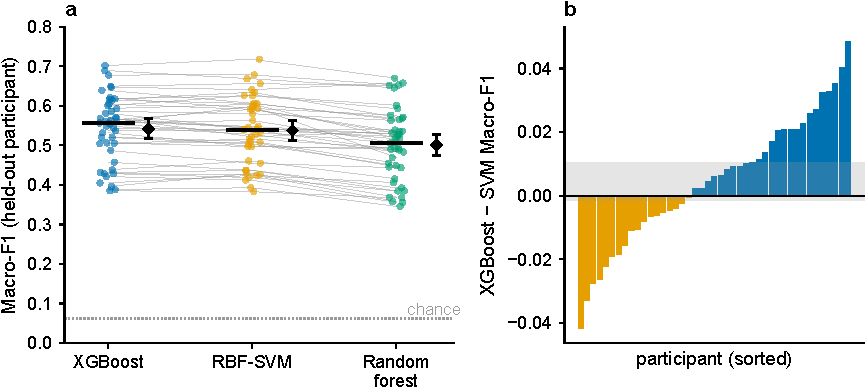
\includegraphics[width=\textwidth]{figures/fig3_full_channel.pdf}
\caption{Full-array leave-one-subject-out performance on GRABMyo (43 participants). (a) Macro-F1 of three classifiers; each point is one held-out participant, grey lines join the same participant, black bars mark medians and diamonds mark means with 95\% cluster-bootstrap confidence intervals. The support vector machine and random forest were trained on samples of 40,000 and 200,000 windows. (b) Paired XGBoost minus support vector machine difference per participant, sorted; the grey band is the 95\% confidence interval of the mean difference.}
\label{fig:full}
\end{figure}

Recognition performance decreased progressively as electrodes were removed (figure~\ref{fig:curve}, table~\ref{tab:sparse_ni}). \chg{The 16-electrode reference of the curve scored \CurveKSixteen, slightly below the full-array result, consistent with the smaller training sample (200,000 windows) shared by all curve models.} Under the prespecified margin of 0.02 Macro-F1, the smallest non-inferior configuration contained $k^* = \KStar$ electrodes. Its mean difference from the corresponding 16-electrode reference was $\DeltaKTwelve$ (95\% CI $\DeltaKTwelveLCB$ to $\DeltaKTwelveUCB$), whereas \chg{the lower confidence bound for 11 electrodes ($\DeltaKElevenLCB$) fell below the margin.} All configurations containing 12--15 electrodes satisfied the criterion, and the minimum acceptable count remained \KStarHolm\ after Holm correction ($k = 12$: $p_{\mathrm{Holm}} \HolmPKTwelve$). As expected, the \chg{minimum count depended on the margin}: the minimum was \KStarMarginPtOne\ electrodes at $\delta = 0.01$ and \KStarMarginPtThree\ at $\delta = 0.03$, again unchanged by Holm correction (supplementary table~S3).

\begin{table*}[t]
\centering
\small
\caption{Electrode-count performance curve and primary non-inferiority decision on GRABMyo (cross-fitted ranking, $\lambda = 0$; 43 participants; every $k$ retrained from scratch on the same 200,000 training windows of each fold). $\Delta_k$: mean paired difference from the $k = 16$ model of the same curve, with 95\% participant cluster-bootstrap confidence interval (CI). Non-inferior: lower bound above $-\delta$ with the primary margin $\delta = 0.02$; Holm: the same decision after Holm correction over the 15 subset sizes. The smallest non-inferior subset ($k^*$) is in bold; the rule below it marks the boundary. Decisions at the sensitivity margins $\delta = 0.01$ and 0.03 are given in supplementary table S3.}
\label{tab:sparse_ni}
\setlength{\tabcolsep}{4pt}
\begin{adjustbox}{max width=\textwidth}
\begin{tabular}{rccccc}
\toprule
$k$ & Macro-F1 (mean $\pm$ SD) & $\Delta_k$ & 95\% CI & Non-inferior & Non-inferior (Holm) \\
\midrule
16 & 0.541 $\pm$ 0.084 & reference &  &  &  \\
15 & 0.538 $\pm$ 0.083 & $-$0.0036 & $-$0.0056 to $-$0.0017 & yes & yes \\
14 & 0.535 $\pm$ 0.083 & $-$0.0060 & $-$0.0081 to $-$0.0039 & yes & yes \\
13 & 0.530 $\pm$ 0.083 & $-$0.0109 & $-$0.0133 to $-$0.0085 & yes & yes \\
\textbf{12} & \textbf{0.528 $\pm$ 0.084} & \textbf{$-$0.0133} & \textbf{$-$0.0160 to $-$0.0106} & \textbf{yes} & \textbf{yes} \\
\midrule 11 & 0.521 $\pm$ 0.084 & $-$0.0204 & $-$0.0246 to $-$0.0162 & no & no \\
10 & 0.515 $\pm$ 0.083 & $-$0.0259 & $-$0.0311 to $-$0.0205 & no & no \\
9 & 0.510 $\pm$ 0.086 & $-$0.0318 & $-$0.0387 to $-$0.0246 & no & no \\
8 & 0.505 $\pm$ 0.085 & $-$0.0366 & $-$0.0440 to $-$0.0289 & no & no \\
7 & 0.500 $\pm$ 0.085 & $-$0.0413 & $-$0.0489 to $-$0.0333 & no & no \\
6 & 0.480 $\pm$ 0.084 & $-$0.0610 & $-$0.0713 to $-$0.0507 & no & no \\
5 & 0.428 $\pm$ 0.075 & $-$0.1133 & $-$0.1277 to $-$0.0993 & no & no \\
4 & 0.397 $\pm$ 0.071 & $-$0.1444 & $-$0.1590 to $-$0.1306 & no & no \\
3 & 0.340 $\pm$ 0.057 & $-$0.2015 & $-$0.2212 to $-$0.1822 & no & no \\
2 & 0.299 $\pm$ 0.057 & $-$0.2420 & $-$0.2603 to $-$0.2230 & no & no \\
1 & 0.181 $\pm$ 0.040 & $-$0.3603 & $-$0.3832 to $-$0.3369 & no & no \\
\bottomrule
\end{tabular}
\end{adjustbox}
\end{table*}


\begin{figure}[t]
\centering
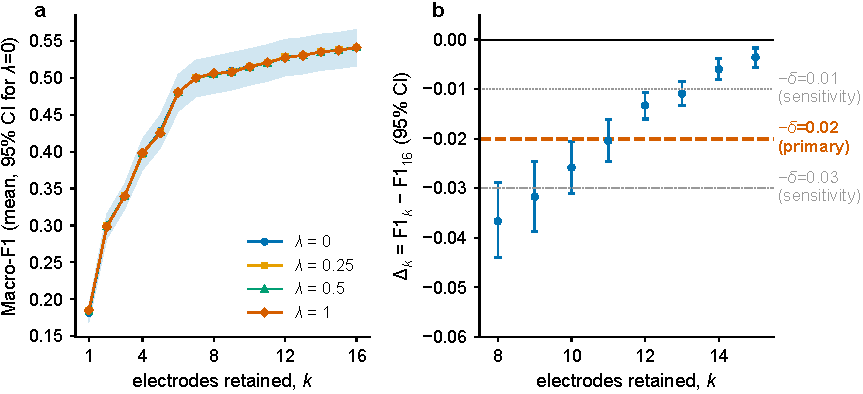
\includegraphics[width=\textwidth]{figures/fig4_sparse_curve.pdf}
\caption{Electrode-count performance curve on GRABMyo (43 participants). (a) Mean Macro-F1 of models retrained on the top-$k$ electrodes of each fold's cross-fitted ranking, for the four values of the stability weight $\lambda$ (the curves overlap); the band is the 95\% cluster-bootstrap confidence interval for $\lambda = 0$. (b) Paired difference to the $k = 16$ model with 95\% confidence interval. The thick dashed line marks the primary margin ($-\delta$, $\delta = 0.02$); the thin dotted and dash-dotted grey lines mark the sensitivity margins (0.01 and 0.03).}
\label{fig:curve}
\end{figure}

Thus, a \KStarReductionPct\% reduction in electrode count was supported within the prespecified engineering tolerance, whereas larger reductions were not. Halving the array to eight electrodes gave a mean difference of $\DeltaKEight$ (95\% CI $\DeltaKEightLCB$ to $\DeltaKEightUCB$), and every reduced configuration had a numerically lower \chg{mean} Macro-F1 than the complete array. Because the ranking was recomputed within every outer fold, this result characterises the electrode count reached by the selection procedure rather than one fixed layout; in practice the procedure excluded the same electrodes (\DroppedFourSet) at $k = 12$ in \DroppedFourFolds\ of 43 folds. \chg{When one 12-electrode layout was instead frozen on half of the participants and tested on the other half, the mean loss was $\FixedDiff$ and $\FixedSwapDiff$ in the two directions; the criterion was met in the first direction and missed narrowly in the second (lower bound $\FixedSwapLCBSix$; supplementary methods~S4).}

\subsection[Evaluation of attribution-guided electrode selection]{Evaluation of attribution-guided electrode selection}
\label{sec:res_attribution}

Both attribution rankings outperformed the mean random-subset baseline at all four tested subset sizes (table~\ref{tab:h2}; 8 tests, Holm-corrected). \chg{The advantage of SR-CFA was largest at six electrodes} ($\HTwoKSixDiff$ Macro-F1, 95\% CI $\HTwoKSixLCB$ to $\HTwoKSixUCB$, $p_{\mathrm{Holm}} \HTwoKSixP$, $r_{rb} = \HTwoKSixR$) \chg{and eight electrodes ($\HTwoKEightDiff$). It was smaller at 12 electrodes ($\HTwoKTwelveDiff$, $p_{\mathrm{Holm}} \HTwoKTwelveP$), where the retained array is close to the full array, and at four electrodes ($\HTwoKFourDiff$).} Cross-fitted SHAP and SR-CFA gave identical results at $k = 6$ and 12 and similar results at $k = 4$ and 8 (table~\ref{tab:h2})\chg{, because the two rankings selected the same subsets for \HTwoSameKSix\ and \HTwoSameKTwelve\ of 43 participants at $k = 6$ and 12 and for \HTwoSameKFour\ and \HTwoSameKEight\ at $k = 4$ and 8}. \chg{Outperforming the mean of the random subsets did not mean outperforming most of them for each participant}: the median percentile of the SR-CFA subset within each participant's random-subset distribution was \PctKFour, \PctKSix, \PctKEight\ and \PctKTwelve\ at $k = 4$, 6, 8 and 12, and it reached the 95th percentile for \PctKAboveNinetyFiveSix\ of 43 participants at $k = 6$ and \PctKAboveNinetyFiveTwelve\ at $k = 12$ (figure~\ref{fig:baselines}(b)).

\begin{table*}[t]
\centering
\small
\caption{\chg{H2: attribution-ranked subsets versus the mean of random subsets of the same size (GRABMyo, 43 participants; secondary family of 8 tests, Holm-corrected; the detailed test family was specified after the underlying results were available). All subsets were evaluated with one comparison model (XGBoost, 50 trees, 150,000 training windows per fold), so absolute values are lower than in table~\ref{tab:sparse_ni}. Random: participant's mean over 100 random subsets (500 at $k = 12$). Difference: mean paired difference (attribution minus random) with 95\% participant cluster-bootstrap confidence interval (CI). Higher/lower: participants for whom the attribution subset scored above/below their random mean. $p_{\mathrm{Holm}}$: Wilcoxon signed-rank, Holm-corrected; $r_{rb}$: matched-pairs rank-biserial correlation.}}
\label{tab:h2}
\setlength{\tabcolsep}{4pt}
\begin{adjustbox}{max width=\textwidth}
\begin{tabular}{rlccccccc}
\toprule
$k$ & Ranking & Attribution & Random & Difference & 95\% CI & Higher/lower & $p_{\mathrm{Holm}}$ & $r_{rb}$ \\
\midrule
4 & Cross-fitted SHAP ($\lambda = 0$) & 0.382 & 0.366 & +0.0163 & +0.0060 to +0.0267 & 29/14 & 0.007 & +0.47 \\
 & SR-CFA ($\lambda = 0.5$) & 0.383 & 0.366 & +0.0172 & +0.0071 to +0.0274 & 30/13 & 0.007 & +0.50 \\
\midrule 6 & Cross-fitted SHAP ($\lambda = 0$) & 0.453 & 0.416 & +0.0370 & +0.0286 to +0.0452 & 37/6 & $<$0.001 & +0.92 \\
 & SR-CFA ($\lambda = 0.5$) & 0.453 & 0.416 & +0.0370 & +0.0286 to +0.0452 & 37/6 & $<$0.001 & +0.92 \\
\midrule 8 & Cross-fitted SHAP ($\lambda = 0$) & 0.468 & 0.445 & +0.0230 & +0.0161 to +0.0298 & 36/7 & $<$0.001 & +0.82 \\
 & SR-CFA ($\lambda = 0.5$) & 0.469 & 0.445 & +0.0243 & +0.0176 to +0.0308 & 37/6 & $<$0.001 & +0.86 \\
\midrule 12 & Cross-fitted SHAP ($\lambda = 0$) & 0.485 & 0.478 & +0.0074 & +0.0046 to +0.0103 & 35/8 & $<$0.001 & +0.71 \\
 & SR-CFA ($\lambda = 0.5$) & 0.485 & 0.478 & +0.0074 & +0.0046 to +0.0103 & 35/8 & $<$0.001 & +0.71 \\
\bottomrule
\end{tabular}
\end{adjustbox}
\end{table*}


In exploratory, uncorrected contrasts (figure~\ref{fig:baselines}(a); supplementary table~S4), no statistically detectable difference between SR-CFA and permutation importance was observed at $k = 4$, 8 or 12 (for example, $k = 8$: $\VSPermKEightDiff$, $p \VSPermKEightP$); at $k = 6$, SR-CFA was higher by $\VSPermKSixDiff$ ($p \VSPermKSixP$). Likewise, no statistically detectable difference between SR-CFA and geometric selection, which spreads electrodes evenly around both rings without using data, was observed at $k = 4$ ($\VSGeomKFourDiff$, $p \VSGeomKFourP$), $k = 8$ ($\VSGeomKEightDiff$, $p \VSGeomKEightP$) or $k = 12$ ($\VSGeomKTwelveDiff$, $p \VSGeomKTwelveP$); at $k = 6$, SR-CFA was higher by $\VSGeomKSixDiff$ ($p \VSGeomKSixP$). Mutual information gave the lowest \chg{mean scores of all methods at every $k \le 8$, below the random-subset mean.}

\begin{figure}[t]
\centering
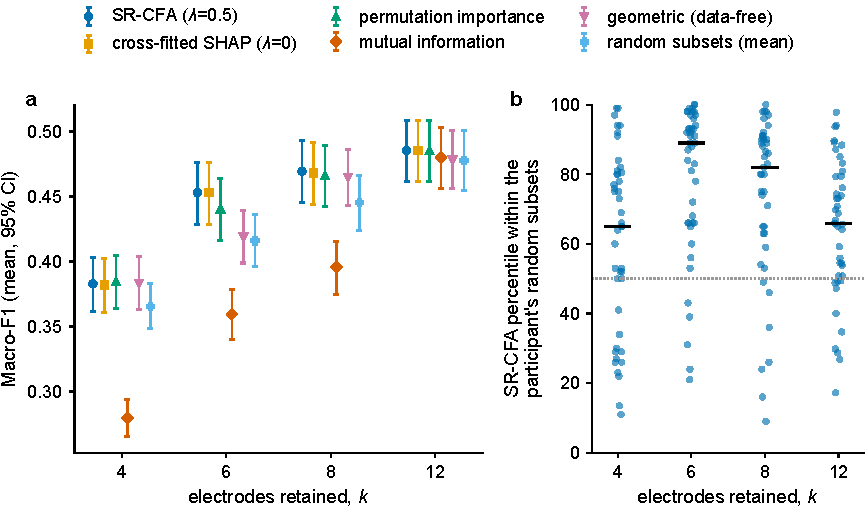
\includegraphics[width=\textwidth]{figures/fig5_selection_baselines.pdf}
\caption{Electrode-selection methods at matched subset size $k$ (GRABMyo, 43 participants; one comparison model shared by all methods). (a) Mean Macro-F1 with 95\% cluster-bootstrap confidence intervals, grouped by method type: attribution rankings (stability-regularised cross-fitted attribution, SR-CFA, and cross-fitted SHAP), model-based rankings (permutation importance and mutual information), data-free geometric selection and the mean over random subsets. (b) Percentile of the SR-CFA subset within each participant's own random subsets (one point per participant; bar = median; 100 random subsets per participant, 500 at $k = 12$).}
\label{fig:baselines}
\end{figure}

Deletion with retraining supported the faithfulness of the ranking (figure~\ref{fig:faithfulness}; supplementary table~S5). Mean Macro-F1 followed the order Remove-Top $<$ Remove-Random $<$ Remove-Bottom at every number of retained electrodes for which all three orders were available, and Remove-Top $<$ Remove-Bottom at every number retained; \FaithNSig\ of the \FaithNTests\ Holm-corrected contrasts were significant. With six electrodes retained, Remove-Top scored \FaithTopKSix, Remove-Random \FaithRandomKSix\ and Remove-Bottom \FaithBottomKSix\ (Remove-Top minus Remove-Random $\FaithTRKSixDiff$, $p_{\mathrm{Holm}} \FaithTRKSixP$; Remove-Random minus Remove-Bottom $\FaithRBKSixDiff$, $p_{\mathrm{Holm}} \FaithRBKSixP$). The separation was largest at intermediate subset sizes and smaller near the extremes, where either very few or nearly all electrodes remained; the Remove-Top versus Remove-Bottom contrast with 14 electrodes retained, where only two electrodes are removed, was not statistically significant ($\FaithTBKFourteenDiff$, $p_{\mathrm{Holm}} \FaithTBKFourteenP$).

\begin{figure}[t]
\centering
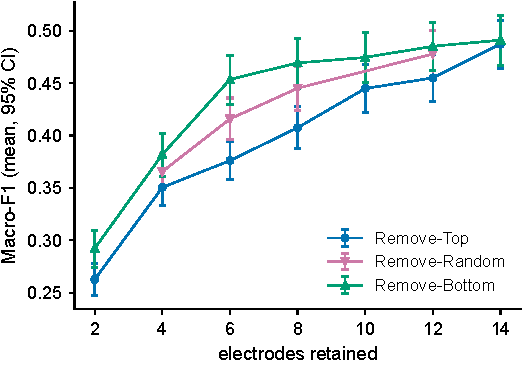
\includegraphics[width=0.62\textwidth]{figures/fig6_faithfulness.pdf}
\caption{Deletion-with-retraining test of attribution faithfulness on GRABMyo (43 participants; mean and 95\% cluster-bootstrap confidence interval). Remove-Top deletes the highest-ranked electrodes, Remove-Bottom the lowest-ranked and Remove-Random a random set; all use the same comparison model and training sample. Remove-Random is shown where random subsets were sampled (4, 6, 8 and 12 electrodes retained).}
\label{fig:faithfulness}
\end{figure}

Stability regularisation did not provide a statistically detectable improvement. Attribution variability across the inner participant groups was small relative to attribution magnitude (median $U_c/A_c$ \UOverAMedian\%, maximum \UOverAMax\%), so positive values of $\lambda$ rarely changed the selected subsets. Relative to $\lambda = 0$, the top-12 set changed in \TopTwelveDiffersLambdaPtTwoFive, \TopTwelveDiffersLambdaPtFive\ and \TopTwelveDiffersLambdaOne\ of 43 folds at $\lambda = 0.25$, 0.5 and 1, and across all four $k$ tested at least \HThreeMinTied\ of 43 participants received the identical subset under both rankings. None of the \HThreeNTests\ contrasts was significant after Holm correction (largest mean difference \HThreeMaxAbsDiff; smallest $p_{\mathrm{Holm}} \HThreeMinP$; supplementary table~S6). The four curves in figure~\ref{fig:curve}(a) differ by at most \LambdaCurveMaxSpread, and $k^*$ was identical under every $\lambda$ and margin; H3 was not supported. A post-hoc participant-level aggregation increased the estimated attribution heterogeneity but did not change $k^*$ under any penalty\chg{; it showed no Holm-corrected difference in performance from fold-level aggregation and no benefit of the penalty within participant-level aggregation} (supplementary methods~S6, table~S7 and figures~S1--S2).

\subsection[Robustness and exploratory analyses]{Robustness and exploratory analyses}
\label{sec:res_exploratory}

Electrode rankings showed substantial agreement across participants, particularly at the upper and lower ends of the ranking (table~\ref{tab:stability}, figure~\ref{fig:attribution}). Rankings computed from individual participants' attributions agreed closely (mean Spearman $\rho$ = \StabSubjRho\ $\pm$ \StabSubjRhoSD\ over \StabSubjPairs\ pairs; mean Jaccard index of the top six \StabSubjJacSix), and rankings from disjoint inner folds agreed at $\rho$ = \StabInnerRho. The same four electrodes (\TopFourSet) formed the top four in \TopFourFolds\ of 43 outer folds and carried \TopFourShare\% of the summed attribution, whereas the eight lowest-ranked electrodes carried \BottomEightShare\%; rank ranges were widest in the middle of the ordering. The outer-fold agreement ($\rho$ = \StabOuterRho) is descriptive only, because those training sets share about 98\% of their participants. \chg{These results indicate} that the subject-independent procedure identified \chg{consistent} spatial preferences, although the data do not support assigning these positions to individual muscles.

\begin{table*}[t]
\centering
\small
\caption{Agreement of electrode rankings on GRABMyo ($\lambda = 0$). Values are mean (SD) over all pairs of rankings in each group. They are descriptive summaries: pairwise observations share rankings and are not independent, so no inferential interval is given.}
\label{tab:stability}
\setlength{\tabcolsep}{4pt}
\begin{adjustbox}{max width=\textwidth}
\begin{tabular}{lcccccc}
\toprule
Rankings compared & Pairs & Spearman $\rho$ & Kendall $\tau$ & Jaccard, top 4 & Jaccard, top 6 & Jaccard, top 8 \\
\midrule
Individual participants & 903 & 0.927 (0.038) & 0.801 (0.066) & 0.752 (0.194) & 0.905 (0.137) & 0.803 (0.132) \\
Inner folds (disjoint participant groups) & 430 & 0.948 (0.021) & 0.840 (0.046) & 0.816 (0.200) & 0.992 (0.047) & 0.838 (0.105) \\
Outer folds (overlapping training sets$^*$) & 903 & 0.987 (0.008) & 0.943 (0.028) & 0.888 (0.180) & 1.000 (0.000) & 0.923 (0.106) \\
\bottomrule
\end{tabular}
\end{adjustbox}
\par\smallskip\parbox{0.95\linewidth}{\footnotesize $^*$Outer training sets share about 98\% of their participants, so their agreement is descriptive only and is not an estimate of between-participant stability.}
\end{table*}


\begin{figure}[t]
\centering
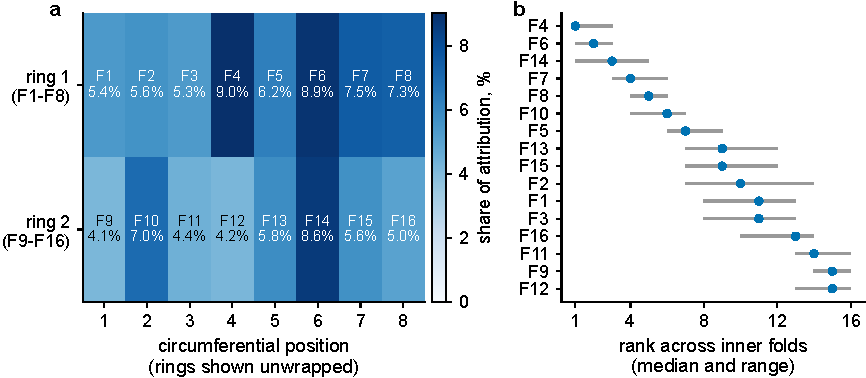
\includegraphics[width=\textwidth]{figures/fig7_attribution.pdf}
\caption{Cross-fitted electrode attribution on GRABMyo ($\lambda = 0$, 43 outer folds). (a) Mean share of attribution per electrode, drawn on the $2 \times 8$ montage; each ring~2 electrode is aligned with, and 2~cm from, the ring~1 electrode at the same circumferential position. (b) Rank of each electrode across inner folds (median and range).}
\label{fig:attribution}
\end{figure}

Replication on NinaPro DB5 was inconclusive. The dataset contained only ten participants and produced substantially wider uncertainty than GRABMyo: full-array Macro-F1 was \DBFiveFull\ $\pm$ \DBFiveFullSD\ (12 movements; chance about 0.083), with between-subject values from \DBFiveFullMin\ to \DBFiveFullMax\ (figure~\ref{fig:generalisation}(b); supplementary table~S8). One reduced configuration ($k = 12$) met the non-inferiority margin by a negligible amount ($\bar\Delta_{12} = \DBFiveDeltaKTwelve$, lower bound $\DBFiveDeltaKTwelveLCBSix$), but the decision was sensitive to Monte Carlo variation in the bootstrap: it was non-inferior in \DBFiveSeedHits\ of \DBFiveSeedN\ bootstrap reruns with different random seeds (\DBFiveSeedFrac\%), a decision-stability diagnostic rather than a probability that the hypothesis is true. Subsets with $k = 13$, 14 and 15 all failed (lower bounds $\DBFiveDeltaKThirteenLCB$, $\DBFiveDeltaKFourteenLCB$ and $\DBFiveDeltaKFifteenLCB$), and no subset remained non-inferior after Holm correction. The replication therefore neither confirms nor contradicts the primary GRABMyo result.

Cross-session analyses provided no evidence of an additional performance loss on later recording days beyond the existing subject-independent gap (figure~\ref{fig:generalisation}(a); supplementary table~S9). Training on session~1 and testing on sessions 1, 2 and 3 gave \CSOneSOne, \CSOneSTwo\ and \CSOneSThree; \chg{session~2 scored higher than session~1} ($\CSSTwoVsSOneDiff$, 95\% CI $\CSSTwoVsSOneLCB$ to $\CSSTwoVsSOneUCB$, uncorrected $p \CSSTwoVsSOneP$), and no statistically detectable difference was observed for session~3 ($\CSSThreeVsSOneDiff$, $p \CSSThreeVsSOneP$). Training on sessions 1 and 2 improved session-3 performance over training on session~1 alone ($\CSTwoVsOneDiff$, 95\% CI $\CSTwoVsOneLCB$ to $\CSTwoVsOneUCB$, $p \CSTwoVsOneP$). However, these contrasts do not isolate electrode displacement, and the apparent benefit of training on two sessions is confounded by the larger amount of training data.

Finally, results from the derived bipolar representation differed from those of the primary monopolar analysis. With the eight derived pairs as the selection unit, full-array Macro-F1 was \BipFull\ $\pm$ \BipFullSD\ for a model trained on all training windows, lower than \chg{the monopolar full-array result} (figure~\ref{fig:generalisation}(c)). As in the monopolar analysis, the reduction curve used a 200,000-window training sample; its $k = 8$ reference scored \BipCurveRefK\ (supplementary table~S10). \chg{The reduction from eight to seven bipolar pairs did not satisfy} the primary non-inferiority criterion ($\bar\Delta_7 = \BipDeltaKSeven$, lower bound $\BipDeltaKSevenLCB$; non-inferior in \BipSeedHitsSeven\ of \BipSeedN\ bootstrap reruns). Under the sensitivity margins, $k^*$ was \BipKStarMarginPtOne\ at $\delta = 0.01$ and \BipKStarMarginPtThree\ at $\delta = 0.03$, identically for all $\lambda$, and pairs \BipTopThreeSet\ formed the top three in \BipTopThreeFolds\ of 43 folds. Consequently, the \KStarReductionPct\% reduction identified in the primary analysis should be interpreted specifically as a reduction in monopolar recording sites on the GRABMyo montage, rather than as evidence that an equivalent proportion of physical bipolar sensors can be removed.

\begin{figure}[t]
\centering
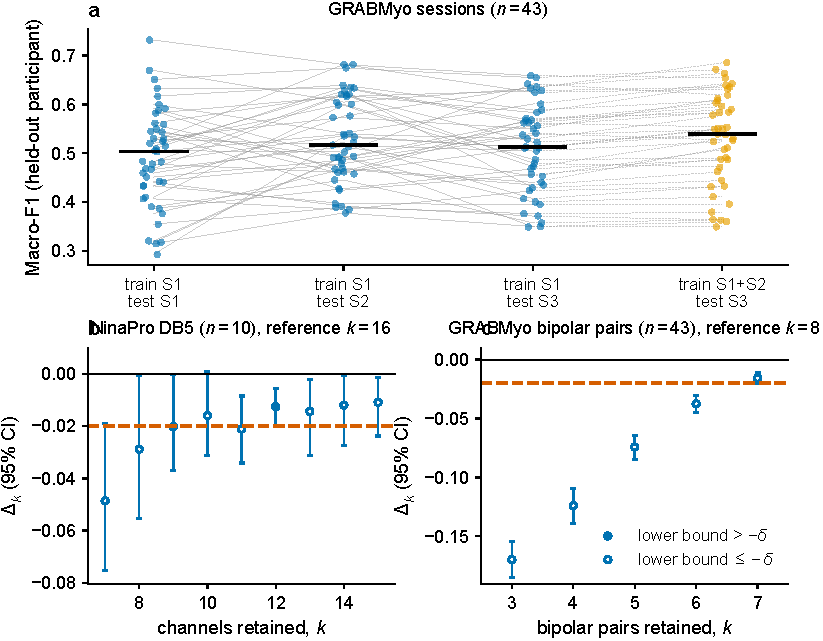
\includegraphics[width=\textwidth]{figures/fig8_generalisation.pdf}
\caption{Exploratory analyses. (a) GRABMyo cross-session evaluation: each point is one held-out participant, grey lines join the same participant across conditions and bars mark medians; every condition is also subject-independent. (b--c) Mean paired difference to the full array of the same curve, $\bar\Delta_k$, with 95\% cluster-bootstrap confidence interval, for (b) NinaPro DB5 (10 subjects, reference $k = 16$), (c) GRABMyo derived bipolar pairs (43 participants, reference $k = 8$). The dashed line marks the primary margin; filled markers indicate a lower bound above the margin and open markers a lower bound at or below it.}
\label{fig:generalisation}
\end{figure}
